\documentclass[11pt]{article}
\usepackage[margin=1in]{geometry}
\usepackage{booktabs}
\usepackage{array}
\usepackage{graphicx}
\usepackage{hyperref}
\usepackage{enumitem}
\usepackage{amsmath}
\usepackage[T1]{fontenc}

\setlength{\parskip}{0.5em}
\setlength{\parindent}{0pt}

\begin{document}

\begin{center}
{\LARGE \textbf{Week 7: Failure Direction Analysis, Activation\\Extraction, and Residual Stream Probing}}
\end{center}

\section*{Project Overview}

This project investigates \textit{where} and \textit{how} commonsense reasoning breaks down inside a large language model. Rather than treating failures on commonsense benchmarks as a black-box data problem, we apply mechanistic interpretability techniques (activation probing, logit lens, and activation patching) to trace failures to specific layers, heads, and representational bottlenecks within the network. The Com2Sense dataset, with its complementary true/false sentence pairs, provides the controlled contrasts needed for causal intervention experiments later in the project.

This second post covers the Week 7 milestone: deepening the complementary pair analysis to quantify failure direction, selecting 200 high-confidence failure pairs for mechanistic work, configuring TransformerLens hooks for residual stream activation extraction, and running linear probes across all 36 layers to localize where the model's commonsense judgments crystallize.

\section*{Experimental Setup}

\textbf{Model.} Qwen/Qwen3-8B, the same instruction-tuned transformer evaluated in Week 6. All activation extraction was performed using TransformerLens's \texttt{run\_with\_cache()} API with a \texttt{names\_filter} restricting cached tensors to \texttt{hook\_resid\_post} at each layer, avoiding the memory cost of storing full attention patterns and MLP intermediates.

\textbf{Dataset.} The 611 asymmetric complementary pairs identified in Week 6 served as the starting pool. From these, 200 pairs were selected for activation extraction based on domain priority and confidence criteria (described below).

\textbf{Activation extraction.} For each of the 200 selected pairs, both the correct and incorrect sentences were run through the model via \texttt{run\_with\_cache()}. At each of the 36 layers, we extracted the residual stream vector at the final token position, producing a tensor of shape [36, 4096] per example, totaling 400 tensors. Extraction ran on an A100-80GB GPU via Modal.

\textbf{Probing.} A logistic regression classifier was trained at each layer to predict a binary label from the [4096] residual stream vector. Cross-validation used \texttt{GroupKFold(n\_splits=5)} with pairs as groups, ensuring that both members of a complementary pair always land in the same fold, preventing leakage from near-duplicate sentences appearing in both train and test.

\section*{Results}

\subsection*{Failure Direction Analysis}

Of the 611 asymmetric pairs from Week 6, we quantified which member the model tends to get wrong, the true statement or the false one:

\begin{center}
\begin{tabular}{l r r}
\toprule
\textbf{Direction} & \textbf{Count} & \textbf{Percentage} \\
\midrule
Failed on TRUE  & 450 & \textbf{73.6\%} \\
Failed on FALSE & 161 & 26.4\% \\
\midrule
\textbf{Total} & 611 & 100\% \\
\bottomrule
\end{tabular}
\end{center}

The model exhibits a strong \textbf{false-bias}: in nearly three-quarters of asymmetric pairs, the model incorrectly labels a true statement as false. This is not a marginal tendency; it is the dominant failure mode across every domain.

\subsection*{Failure Direction by Domain}

\begin{center}
\begin{tabular}{l r r r r}
\toprule
\textbf{Domain} & \textbf{Failed on TRUE} & \textbf{Failed on FALSE} & \textbf{Total} & \textbf{\% Failed on TRUE} \\
\midrule
Social   & 162 & 46 & 208 & \textbf{77.9\%} \\
Physical & 125 & 44 & 169 & 74.0\% \\
Time     & 111 & 46 & 157 & 70.7\% \\
Temporal &  52 & 25 &  77 & 67.5\% \\
\bottomrule
\end{tabular}
\end{center}

The false-bias is strongest in the social domain (77.9\%) and weakest in temporal (67.5\%), but present everywhere. Social-causal is the most extreme subcategory: \textbf{87.0\%} of its asymmetric failures are on true statements.

\subsection*{Failure Direction by Domain + Scenario}

\begin{center}
\begin{tabular}{l r r r r}
\toprule
\textbf{Subcategory} & \textbf{Failed on TRUE} & \textbf{Failed on FALSE} & \textbf{Total} & \textbf{\% Failed on TRUE} \\
\midrule
Social-Causal       & 87 & 13 & 100 & \textbf{87.0\%} \\
Physical-Causal     & 73 & 22 &  95 & 76.8\% \\
Time-Causal         & 57 & 23 &  80 & 71.2\% \\
Time-Comparison     & 54 & 23 &  77 & 70.1\% \\
Social-Comparison   & 54 & 22 &  76 & 71.1\% \\
Physical-Comparison & 37 & 13 &  50 & 74.0\% \\
Temporal-Causal     & 29 & 11 &  40 & 72.5\% \\
Temporal-Comparative& 22 & 14 &  36 & 61.1\% \\
Social-Comparative  & 21 & 11 &  32 & 65.6\% \\
Physical-Comparative& 15 &  9 &  24 & \textbf{62.5\%} \\
\bottomrule
\end{tabular}
\end{center}

Causal subcategories consistently show the strongest false-bias (76--87\%), while comparative subcategories show the weakest (61--66\%). This suggests that the model's tendency to reject true statements is amplified when it must evaluate causal chains rather than direct comparisons.

\subsection*{Selection of 200 High-Confidence Failure Pairs}

From the 611 asymmetric pairs, we selected 200 for activation extraction using the following criteria:

\begin{enumerate}[leftmargin=2em]
\item \textbf{Domain priority.} Pairs from the lowest-accuracy domains (temporal: 63.5\%, time: 66.6\%) were included first.
\item \textbf{Confidence threshold.} Only pairs where the model's confidence on the wrong answer exceeded 0.70 were included, as these are cases where the model was decisively wrong, not borderline.
\item \textbf{Logit gap threshold.} A minimum logit gap of 1.0 between the True and False tokens ensured a strong but incorrect signal.
\end{enumerate}

After exhausting temporal and time pairs meeting these criteria, social-domain pairs were added until 200 were reached. Physical-domain pairs were not needed.

\begin{center}
\begin{tabular}{l r}
\toprule
\textbf{Domain} & \textbf{Selected Pairs} \\
\midrule
Time     & 103 \\
Temporal &  50 \\
Social   &  47 \\
\midrule
\textbf{Total} & \textbf{200} \\
\bottomrule
\end{tabular}
\end{center}

The selected set has an average confidence on the wrong answer of \textbf{0.896} and an average logit gap of \textbf{2.534}, ensuring that the activation extraction targets the model's most confident failures rather than noisy borderline cases. Within the selected 200, 153 pairs (76.5\%) failed on the true statement and 47 (23.5\%) failed on the false statement, roughly consistent with the overall false-bias observed across all 611 asymmetric pairs.

\subsection*{Activation Extraction via TransformerLens Hooks}

For each of the 200 selected pairs, both the correct and incorrect sentences were passed through Qwen3-8B using TransformerLens's \texttt{run\_with\_cache()} with a \texttt{names\_filter} that caches only \texttt{hook\_resid\_post} at each layer. At every layer, the residual stream vector at the final token position was extracted and moved to CPU, yielding a tensor of shape [36, 4096] per example. This produced 400 tensors stored in a single \texttt{activations.pt} file alongside an \texttt{activations\_meta.json} recording pair metadata, model configuration, and run information.

Prior to the full extraction run, we verified that the hook-based caching works correctly by running a test forward pass and confirming that \texttt{resid\_post} at each of the 36 layers returns the expected shape of [1, sequence\_length, 4096]. This verification step was added to the project's smoke test suite so that any future model or TransformerLens version change will be caught before a full extraction run.

The \texttt{names\_filter} approach is critical for memory efficiency: caching only \texttt{resid\_post} avoids storing attention patterns, MLP intermediates, and other hook points that would multiply GPU memory usage by roughly 10$\times$.

\subsection*{Linear Probing Results}

Three linear probes were trained across all 36 layers:

\begin{center}
\begin{tabular}{l r r}
\toprule
\textbf{Probe} & \textbf{Best Layer} & \textbf{Best Accuracy} \\
\midrule
Correctness (no PCA)    & 32 & 54.75\% \\
Correctness + PCA-50    & 30 & \textbf{61.00\%} \\
Ground truth + PCA-50   & 31 & 60.00\% \\
\bottomrule
\end{tabular}
\end{center}

\textbf{Probe 1: Correctness, no PCA.} Label: $y{=}1$ if the model answered correctly, $y{=}0$ if incorrectly. Features: raw [4096] residual stream vector, standardized. This probe asks whether the residual stream linearly predicts model behavior.

\textbf{Probe 2: Correctness + PCA-50.} Same label as Probe 1, but features are first reduced to 50 principal components (fit on training folds only). With ${\sim}320$ training examples in a 4096-dimensional space, the problem is severely underdetermined. Compressing to 50 components keeps the most variance-explaining directions and strips out noise, giving logistic regression a tractable problem.

\textbf{Probe 3: Ground truth + PCA-50.} Label: $y{=}1$ if the statement is true, $y{=}0$ if false (the actual ground truth, regardless of what the model predicted). This asks a purer question: does the residual stream encode the correct answer at all, independent of the model's output?

All three probes are at chance (${\approx}50\%$) through \textbf{layers 0--19}, then rise consistently from \textbf{layer 20 onward}, peaking in the \textbf{23--32 range}.

\begin{center}
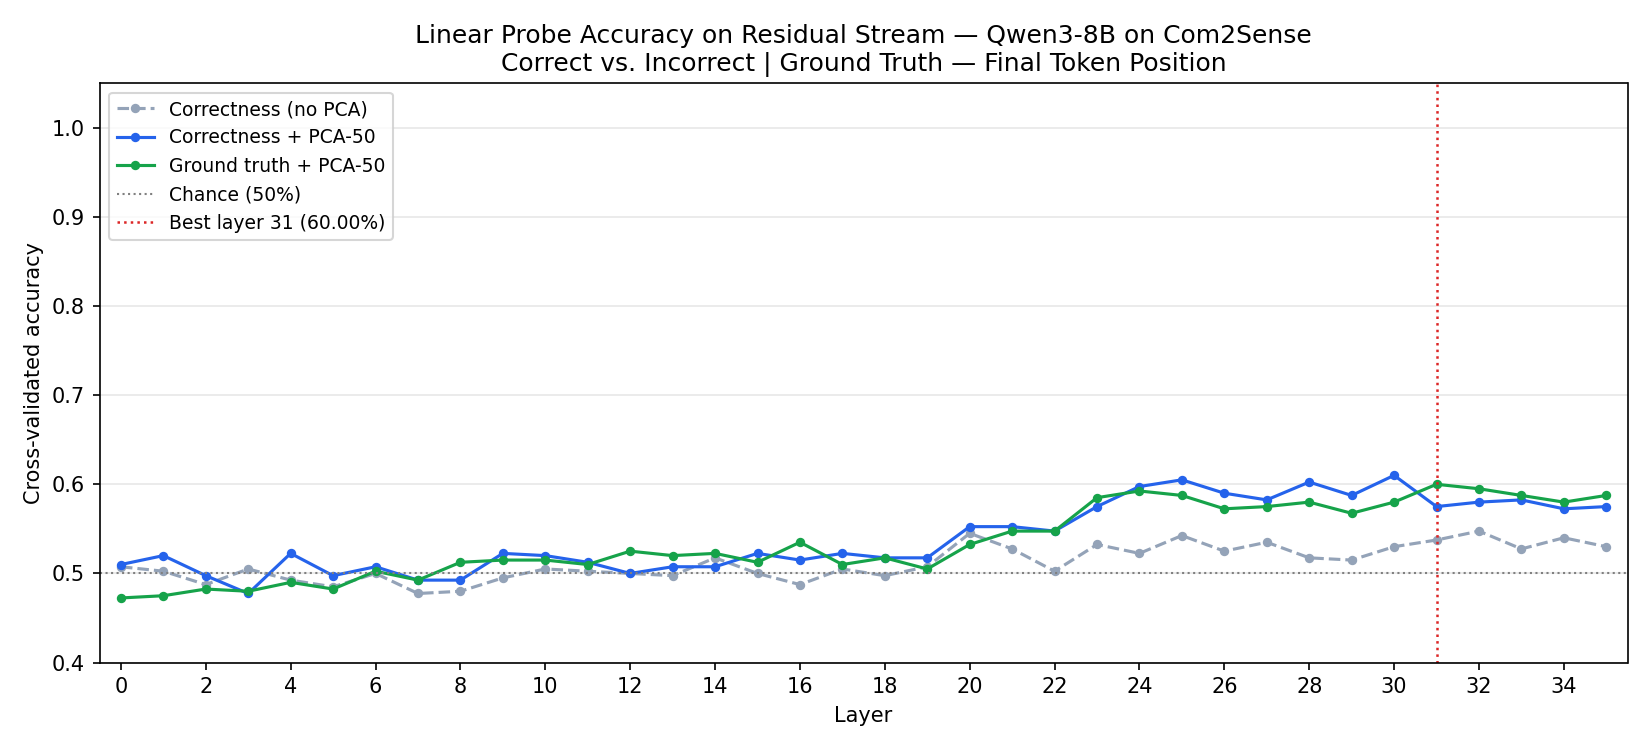
\includegraphics[width=\textwidth]{reports/figures/probe_accuracy_curve.png}
\end{center}

\subsection*{Per-Domain Accuracy at Best Layer}

At layer 31 (best for the ground truth + PCA-50 probe):

\begin{center}
\begin{tabular}{l r}
\toprule
\textbf{Domain} & \textbf{Probe Accuracy} \\
\midrule
Time     & 60.2\% \\
Social   & 59.6\% \\
Temporal & 57.0\% \\
\bottomrule
\end{tabular}
\end{center}

The domain ranking mirrors the Phase 1 accuracy rankings: temporal reasoning is not only the most error-prone domain but also the hardest to linearly separate in the residual stream.

\section*{Discussion}

\textbf{The model has a systematic false-bias.} The failure direction analysis reveals that 73.6\% of asymmetric failures occur on true statements. The model is not failing randomly within pairs: it systematically tends to label true statements as false. This bias is strongest in causal scenarios (up to 87\% in social-causal), suggesting that when evaluating causal chains, the model defaults toward rejection. This is a structural tendency in the model's reasoning, not a property of the dataset.

\textbf{Physical-causal is not the hardest subcategory, contrary to our initial hypothesis.} In our project proposal, we predicted that physical-causal reasoning would produce the highest failure rate, expecting that causal chains involving physical objects would be particularly challenging. The data show the opposite: physical-causal accuracy is 74.0\%, well above the overall average of 70.25\%. The hardest subcategories are temporal-comparative (60.7\%) and time-comparison (65.3\%). In retrospect, this makes sense: physical causal facts (e.g., ``heavier objects are harder to lift'') frequently appear in pretraining data in explicit, rule-like forms, making them relatively easy for the model to retrieve. Temporal and comparative reasoning, by contrast, require implicit integration of durations, sequences, and magnitudes that are rarely stated directly in text. We have verified the evaluation setup is correct (the smoke test confirms token verification, forward pass shapes, and hook extraction), so the discrepancy reflects a genuine property of the model rather than a methodological error.

\textbf{Commonsense judgment forms late in the network.} The probing results show a clear phase transition around layer 20. The first 19 layers (more than half the network) carry no linearly separable signal for either correctness or ground truth. The features that distinguish correct from incorrect reasoning crystallize only in the back half of the model, consistent with prior work showing that factual and reasoning computations occur in later transformer layers.

\textbf{PCA reveals signal that raw probing misses.} The jump from 54.75\% (no PCA) to 61.00\% (PCA-50) on the same correctness label shows that the signal is real but sparse relative to the 4096-dimensional space. With only 400 examples, a linear classifier overfits to noise in the full space; compressing to 50 principal components exposes the meaningful directions.

\textbf{The model is representationally committed to wrong answers.} Correctness is slightly more separable than ground truth (61\% vs.\ 60\%). The residual stream more cleanly encodes \textit{what the model will predict} than \textit{what the correct answer is}. This rules out a simple ``the model knows the answer but randomly outputs the wrong token'' story; the commitment to the wrong answer is already present in the residual stream before the final projection.

\textbf{Temporal reasoning failures are the least structured.} Domain probe accuracy at the best layer mirrors Phase 1 behavioral accuracy: time (60.2\%) $>$ social (59.6\%) $>$ temporal (57.0\%). Temporal failures are not only more frequent but also less linearly separable, suggesting a more distributed or inconsistent failure mode in the residual stream.

\textbf{The signal is weak overall (${\approx}61\%$).} Even at the best layer with PCA, accuracy is well below what strong probes on clear factual tasks typically achieve (often 80--95\%). This could indicate that the distinction between correct and incorrect commonsense reasoning is genuinely diffuse, that the final token position is not the richest probe site, or that 200 pairs provide insufficient training data even with dimensionality reduction.

\section*{Next Steps (Week 8)}

\begin{itemize}[leftmargin=2em]
\item Run \textbf{activation patching} experiments targeting layers 20--32, swapping the residual stream between correct and incorrect examples within each pair to identify which layers causally control the model's commonsense output.
\item Perform \textbf{head-level patching} within the critical layers to isolate specific attention heads responsible for reasoning failures, particularly in the temporal domain where layer-level probing shows the least structure.
\item Explore probing at \textbf{intermediate token positions} (over the statement itself, not just the final token) to test whether stronger signal exists earlier in the sequence.
\end{itemize}

\end{document}
